\documentclass{article}
\usepackage[utf8]{inputenc}
\usepackage[english]{babel}
\usepackage{titlepic}
\usepackage{blindtext}
\usepackage{graphicx}
\usepackage{url}
\usepackage{hyperref}
\usepackage{multirow}
\usepackage[section]{placeins}
\usepackage[style=ieee]{biblatex}
\addbibresource{refs.bib}

\graphicspath{{./images/}}

\title{Chess Engine AI}
\author{Author: Leon Szabo (201515134)}
\date{Project Supervisor: Flávia Alves}
\titlepic{
\includegraphics[width=0.8\textwidth]{uol}}

\begin{document}

\maketitle

\newpage
\tableofcontents

\newpage
\section{Project Description} \label{description}
The popular board game chess has recently gained a surge in popularity\cite{popularity} with new players looking to improve their skills. As a result, chess engines are needed more than ever so that players can improve their skills by analysing misplays in games in an offline setting. That is especially the case for players at the highest level, where a game analysis tool can significantly decrease the time required to look through the possible move variations and find which moves with slight game variations are better than looking through the possible moves without an AI system.

The chess engine AI we plan to create aims to provide a GUI with a competitive algorithm that will allow players to challenge the AI. We will write the back-end and front-end in Go, using the Fyne\cite{fyne} package for the GUI. As for the chess engine's search and evaluation, we will use alpha/beta algorithms.

\section{Aims \& Objectives}
\subsection{Aims:}
\begin{itemize}
    \item Program a chess engine
    \item Create a stylistic and simple GUI
    \item Add player vs AI compatibility
\end{itemize}

\subsection{Objectives:}
\begin{itemize}
    \item Develop a chessboard representation
    \item Develop a chess search and evaluation algorithm
    \item Implement automated testing through GitHub
    \item Evaluate performance of chess engine
    \item Add intractability to GUI
\end{itemize}


\section{Key literature \& Background Reading}
There have been many chess engine creations over the years, and with every year, resources have expanded, and knowledge about chess and AI has furthered. 

The first part of creating a chess engine is the board representation, a way to characterise how a computer sees the board and where the pieces are. There are two categories that representation falls into, piece-centric and square-centric\cite{chessprog:board}. Square-centric styles tend to be simple; they also tend to be slower and more inefficient. Therefore, piece-centric styles are preferred as they offer a better way to evaluate chess positions giving a considerable performance benefit over square-centric models. Bitboards fall in the piece-centric class\cite{craftychess:board}.

After board representation, there is the search and evaluation. Depth-First search is a commonly used category of search algorithms; other algorithms, like Breadth-First, try to explore the whole domain of possible moves; in a game like chess, an estimated \(10^{43}\)\cite{history:search} possible positions is not feasible for an algorithm to process. So instead, Depth-first aims to explore each branch before backtracking; we will use alpha-beta, a commonly used expandable Depth-first search algorithm\cite{chessprog:search}.

\section{Development \& Implementation Summary} \label{imp}
The development environment we will be using is Visual Studio Code\cite{vscode}, as I have used it throughout my course and have become comfortable with it. Another reason for its usage is that it natively supports various languages, including Go\cite{vscode:languages}, the programming language we will be using. We are using Go because the language is fast, simple, and maintainable\cite{Go:popularity}; I have also become fond of the language as it has many features that make it easy to write and maintain, such as the built-in testing library\cite{golang}.\\

\noindent\textbf{1. Create Chess board representation and rules:}\\
Board representation is needed to evaluate moves, detect attacks, and hold positions. In essence, it is the backbone of the engine. Therefore, having a good board representation is essential. So we plan to \emph{create a bitboard} and \emph{use bit operations}\cite{craftychess:board} for the rules of Chess.

\noindent\textbf{2. Program Chess AI:}\\
There are two main types of chess AI: hand-crafted evaluation (HCE) and multi-layer neural networks\cite{chessprog:eval}. We will be \emph{making an HCE algorithm using minimax and alpha-beta pruning}.

\noindent\textbf{3. Create a stylish and simple GUI:}\\
All chess engines incorporate similar placements of GUI elements\cite{chess.com}\cite{lichess}\cite{chess24}; the chess board on the left, taking up the majority of the screen; and the point value of the winning side on the top right. For the standard, \emph{we will be using the same placements}. For the style, \emph{we will use a minimalistic GUI.}

\noindent\textbf{4. Add player vs AI compatibility:}\\
Before adding this compatibility, we must have already finished the AI vs AI compatibility. Adding AI vs player compatibility will require \emph{being able to move the chess pieces} and \emph{adding a helper line} to show where the pieces clicked on can move, among other features.

\noindent\textbf{5. Evaluate the performance of the AI:}\\
After the chess engine's creation, it will be \emph{tested against chess engines of increasing difficulty} to get game outcomes in a parsable format. A ranking algorithm such as Ordo\cite{ordo} can then \emph{work out its rating against other chess engines} by receiving a PGN\cite{wiki:PGN} as input and calculating a rank based on the results of what the PGN contains.

\section{Data Sources} % TODO UNCHECKED
The only data source we plan to use is from the CCRL website\cite{ccrl}; it is a list of chess engines and their calculated ratings by the CCRL testing group; from this list, we will only be using the free or open-source engines. There is more detail on how we plan to use the engines in section \ref{Eval}.

\section{Testing \& Evaluation} % TODO UNCHECKED
\subsection{Testing:}
Most of the testing will be automated rather than manually tested, as having a quick way to check if certain functionalities of the chess engine work is better than manually checking them each time we make an edit. In addition, Go, the programming language we will be using, has a built-in testing package, making it easy to incorporate while programming to test semantic errors. Finally, Visual Studio code will catch most syntax errors.

We will be implementing unit testing, integration testing, and GUI testing. Unit testing is essential to ensure all back-end functions work as intended isolated. Integration testing is just as necessary as functions working in isolation will not mean they work together. Go's testing package can be used to automate both of these testing methods; we will be able to program alongside testing with Github actions.

GUI testing is much harder to automate; depending on the scale of the GUI we implement, it may be automated or manually tested. If we decide to use automation, we will use AutoHotKey\cite{AHK} to simulate user actions.

\subsection{Evaluation:} \label{Eval}
On top of testing the code, we will need to evaluate the strength of the chess engine to see if it performs well. There are two routes to take with evaluation; we could introduce human participants that could play against the AI or introduce another chess engine to play against our AI.

Introducing human participants will bring complications, such as how good a chess player thinks they are against how well they play in reality. There may also not be players good enough to play against the AI and adequately determine its strength; collecting and compiling data may also prove to be time-consuming. That is why we decided to take the AI vs AI route; pitting our AI against already-established engines that have an evaluated rank will significantly increase the precision of our evaluation.

We will start our evaluation by fetching a list of free or open-source engines and their ratings from the CCRL website\cite{ccrl}. Then pit them against each other using Cute Chess's\cite{cutechess} AI vs AI capability to generate PGNs, which can be parsed through Ordo\cite{ordo} to generate a ranking.

\section{Ethical Considerations}
Currently, there is nothing that would require us to act ethically. However, we have read the ethical considerations and will follow them if we make changes.

\section{BSC Project Criteria} % TODO UNCHECKED
\noindent\textbf{An ability to apply practical and analytical skills gained during the degree programme:}\\
I have learned a lot over the degree programme, with many practical programming skills coming from nearly all courses in years one and two. Analytical skills have also come from programming, as problem-solving is fundamental to programming.

\noindent\textbf{Innovation and/or creativity:}\\
As no program is the same, Innovation will come from programming the back end, especially the AI aspect of the chess engine; we will need to innovate for the chess engine to perform well. In addition, we need to be creative if we want to experiment with AI, and as the chess engine has GUI implementation, design choices will require creativity.

\noindent\textbf{Synthesis of information, ideas and practices to provide a quality solution together with an evaluation of that solution:}\\
There are many resources for chess engines; we will research and apply analytical skills to summarise it into something manageable. As mentioned in section \ref{Eval}, we will be using Ordo\cite{ordo} and Cute Chess\cite{cutechess} for the evaluation.

\noindent\textbf{"That your project meets a real need in a wider context.":}\\
As mentioned in section \ref{description}, players use chess engines for analysis; engines significantly decrease the time needed to calculate possible board variations.

There is also a need to make competing software to increase chess engine quality. Without competition, there would be a lack of strong chess AI.

\noindent\textbf{"An ability to self-manage a significant piece of work.":}\\
Following the Gantt chart in section \ref{plan} will allow us to see where we are in the project and track our progress to see if we are falling behind. I have learned how to manage time by keeping to deadlines; this skill will allow us to segment work and produce results on dates throughout the project.

\noindent\textbf{"Critical self-evaluation of the process.":}\\
When we finish major parts of the project, such as the bitboard creation, auto testing, and the GUI. We will see what has been successful or unsuccessful and improve what we have built.

\section{UI/UX Mockup} % TODO WIP
As mentioned in section \ref{imp}.3, chess engines, for the most part, incorporate similar GUI placements; if we decide to defer from the standard, it would have to be for a good reason. Changing it might confuse chess players who are used to the standard placements. That is why we decided to stick to the standard with a reasonably simple GUI, as seen in figure \ref{fig:gui}

The chess board is on the left side, taking up most of the space; this is where the player can interact with the pieces; The figures chess board is from Lichess\cite{lichess}. Our GUI will have a similar style but might use different chess piece designs depending on what we think looks better. The right side shows the chess piece move history in algebraic notation\cite{wiki:algebra}. As our GUI is straightforward now, if we have extra time to work on optional features such as game look back, we can quickly implement them into the GUI as there is plenty of white space.
\begin{figure}[!htb]
    \centering
    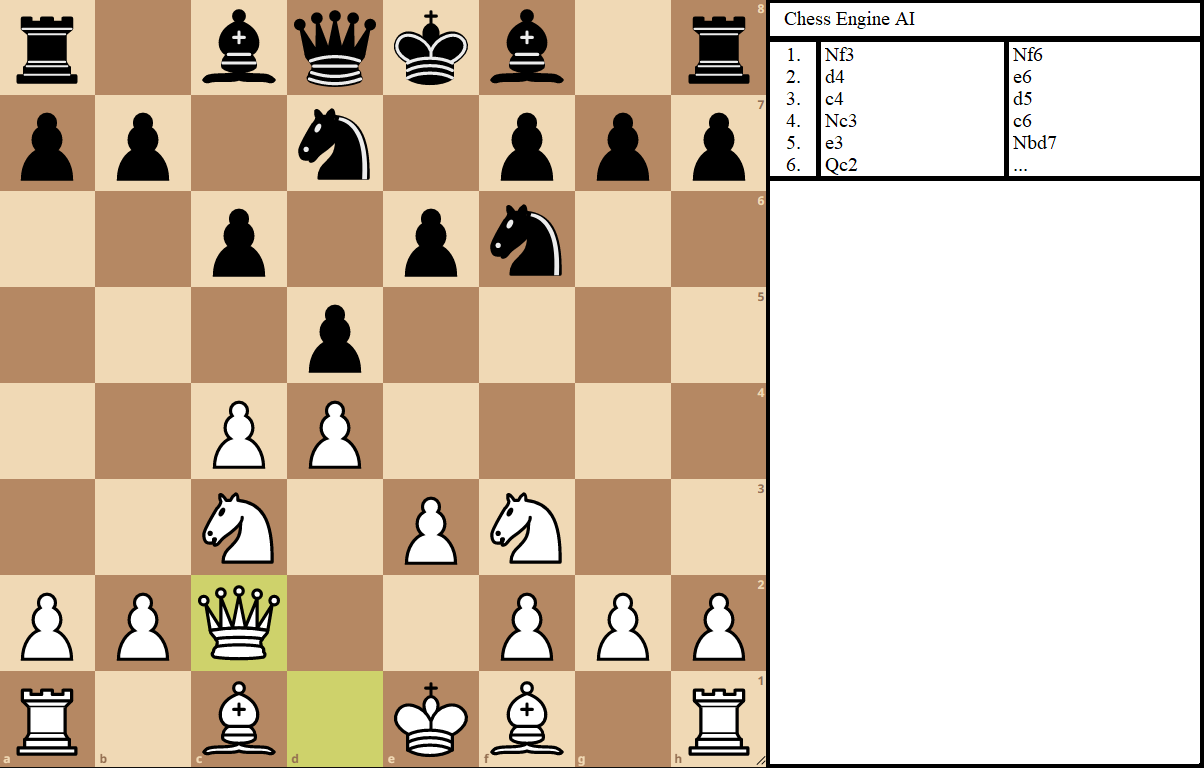
\includegraphics[width=1\textwidth]{GUI}
    \caption{Example GUI for chess engine, adapted from Lichess\cite{lichess}}
    \label{fig:gui}
\end{figure}

\newpage
\section{Project Plan} \label{plan} % TODO WIP
We have laid out the project plan as a Gantt chart created in Instagantt\cite{gantt}; there are three main focuses, the bitboard, auto-testing, and GUI creation; we will start writing the honours halfway through the course when there is enough material to start.

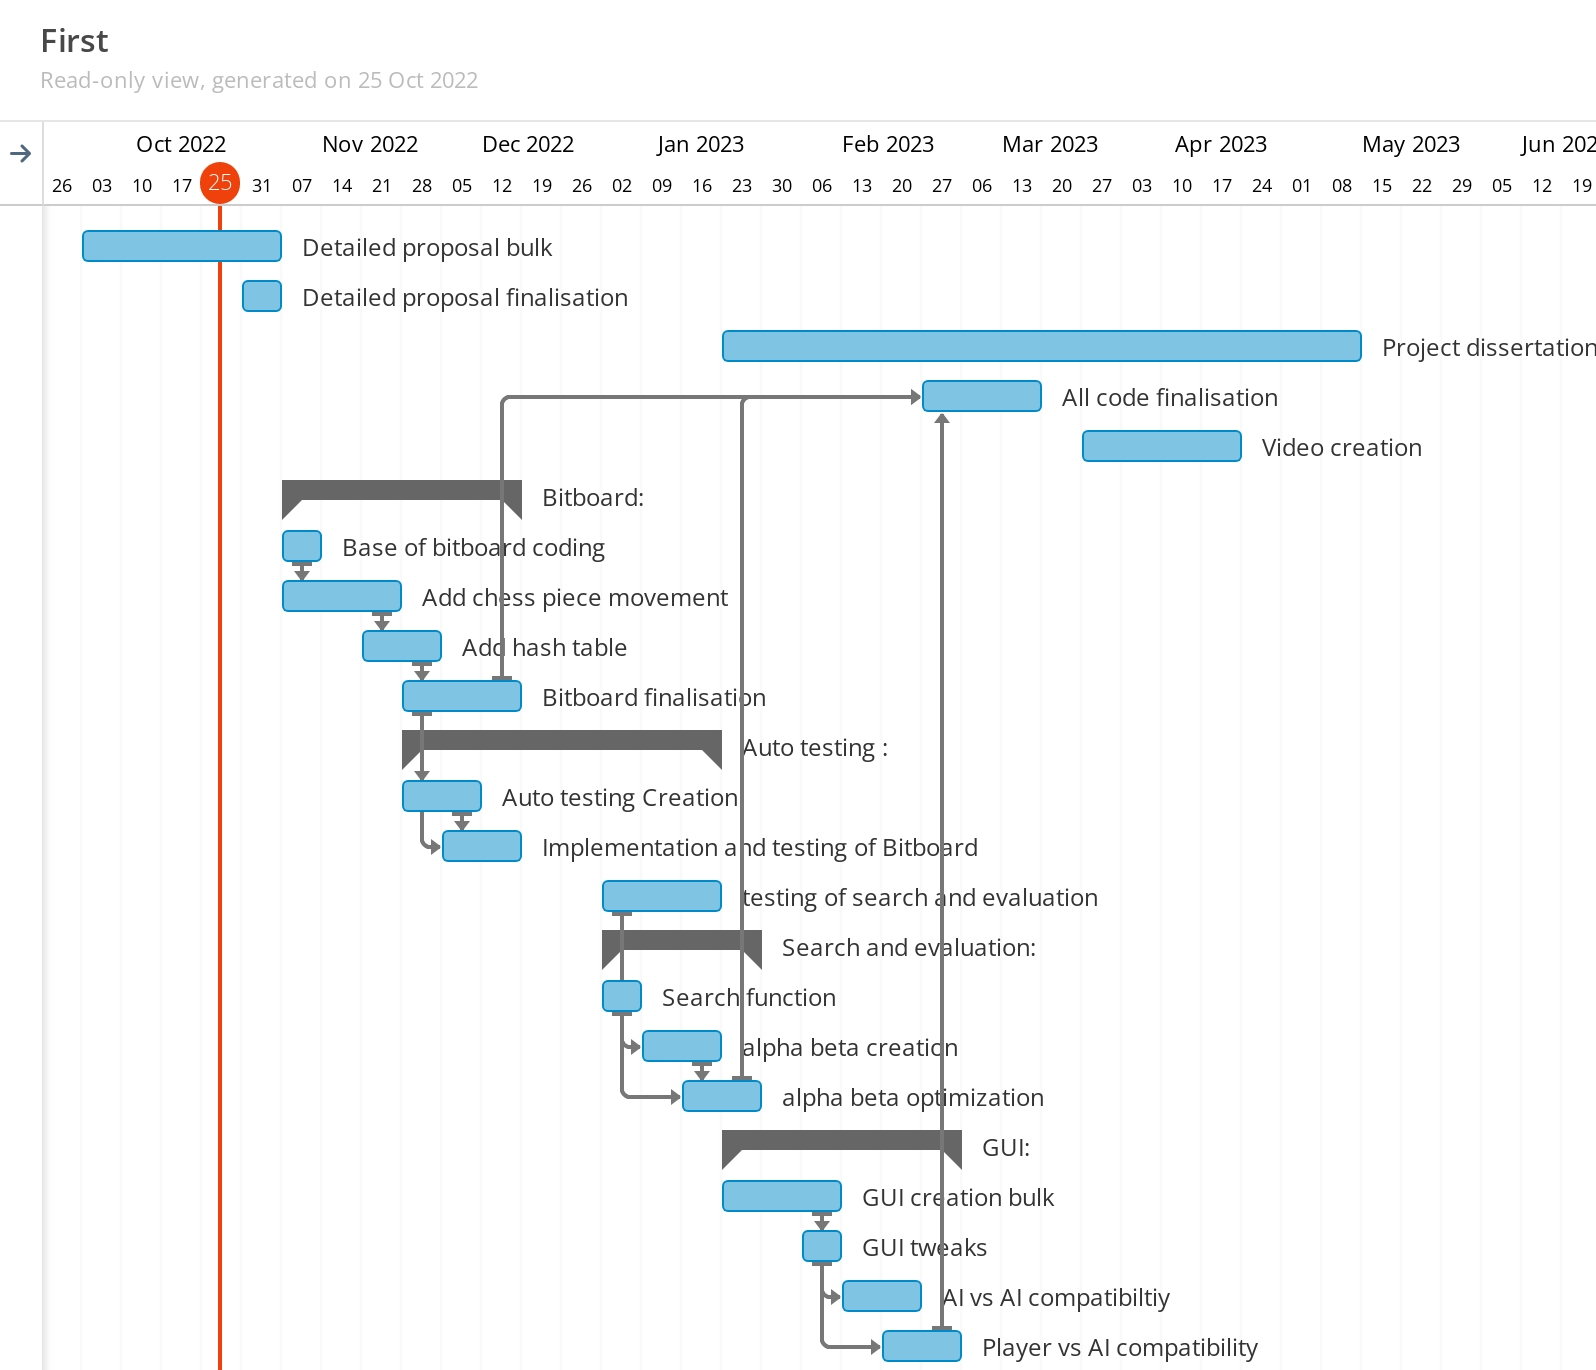
\includegraphics[height=90mm,width=0.95\textwidth]{ProjectPlan}

\section{Risks and Contingency plans} % TODO UNCHECKED
\begin{tabular}{|p{0.21\textwidth}|p{0.21\textwidth}|p{0.21\textwidth}|p{0.21\textwidth}|}
    \hline
    \multicolumn{4}{|c|}{Plans}\\
    \hline
    Risks & Contingencies & Likelihood & Impact\\
    \hline
    Producing broken code & Regularly test code & high. There will be a lot of code, we are bound to make mistakes & low. we plan to remove all errors through testing\\
    \hline
    Low productivity & Have regular check-ins & medium. We will have to balance working on this and other things & medium. This will impact us if we miss a week or two and fall behind\\
    \hline
\end{tabular}
\\
\begin{tabular}{|p{0.21\textwidth}|p{0.21\textwidth}|p{0.21\textwidth}|p{0.21\textwidth}|}
    \hline
    Risks & Contingencies & Likelihood & Impact\\
    \hline
    Forgetting to save & Make regular backups of work & low. our IDE implements autosaving so saving is still quite frequent & low. auto saves are frequent so there won't be that much loss\\
    \hline
    Drive failure & Make regular off-site backups on Github & low. Drives do not usually fail & high. Could be detrimental if we have not made backups\\
    \hline
    Inaccurate deadlines from Gantt chart & Produce working code at the minimum & low. In nearly all cases overestimations have been made & high. It could delay us by weeks if estimations aren't accurate\\
    \hline
\end{tabular}

\newpage % References
%\bibliographystyle{IEEEtran}
%\bibliography{refs}
\printbibliography

\end{document}
